\chapter{Einleitung}\label{einleitung}
In der heutigen Zeit gewinnen Videospiele immer mehr an Bedeutung und verdrängen dabei zunehmend klassische Medien der Entertainment-Branche. So hat der bisher finanziell erfolgreichste Film \Fachbegriff{Avengers: Endgame} insgesamt einen Umsatz von etwa \$2,8 Milliarden erzielt \cite{endgame}; das Spiel \Fachbegriff{Grand Theft Auto V} hingegen konnte mehr als \$6 Milliarden \cite{gta5} und \Fachbegriff{World of Warcraft} sogar Einnahmen von \$9,23 Milliarden bereits im Jahr 2016 \cite{wow} erzielen. Mit der steigenden Relevanz des Marktes sowie dem verfügbaren Kapital in der Branche steigen ebenfalls die Erwartungen der Spieler an das Spielerlebnis. Auf dem visuellen Level äußert sich dies in einer stetig verbesserten Grafikqualität und damit verbundenen höheren Hardwareanforderungen.

Gleichzeitig ist ein ähnlich großes Wachstum in der Machine Learning-Branche zu verzeichnen. Gestiegene Möglichkeiten und kontinuierliche Entwicklungen besonders im Bereich des \Fachbegriff{Deep Learning} haben dazu geführt, dass immer mehr Firmen vermehrt auf \Fachbegriff{Künstliche Intelligenz} bauen und KI-gestützte Prozesse für intelligentere Verfahren verwenden. Kürzliche Erfolge haben gezeigt, dass mit Technologien wie \Fachbegriff{Reinforcement Learning} Systeme entwickelt werden können, deren Intelligenz in ihrem Expertenbereich über die kognitiven Fähigkeiten von menschlichen Anwendern und selbst professionellen Esports-Spielern hinausgeht \cite{openai_five_win}. Somit wurden auch in der Spieleindustrie Durchbrüche erzielt.

Im Vergleich zu älteren Spielen haben heutige \acp{npc} hinsichtlich ihrer Glaubwürdigkeit eine enorme Steigerung erfahren. Generell konnte die Qualität und Überzeugungsfähigkeit virtueller Spielwelten seit der Popularisierung von Videospielen kontinuierlich gesteigert werden. Der hohe grafische Standard erzeugt dabei gerade in Verbindung mit neuen Technologien wie \Fachbegriff{Virtual Reality} aber auch einen hohen Erwartungslevel an die Authentizität von \acp{npc} \cite{skyrim_cif-ck_paper}. Der Kontrast zwischen visueller Qualität und der Authenzität der Umgebung des Spielers steht allerdings im direkten Konflikt zu den Erwartungen der Spieler.
Bei näherer Betrachtung zeigen diese häufig trotz der Verbesserungen einen sehr niedrigen Level von Dynamik und Lebendigkeit. Für sich betrachtet wirken einzelne \acp{npc} häufig berechenbar und wenig eigenständig, obwohl die Atmosphäre eines Spiels maßgeblich davon abhängt, wie lebendig diese wirken. Die Glaubwürdigkeit der Umgebung des Spielers wird direkt durch die gewählten Aktionen eines \acp{npc} beeinflusst und erhöht sich mit einem möglichst menschlich wirkenden Verhalten. Dazu zählen nicht nur interaktionsfähige \acp{npc} sondern ebenfalls Hintergrundcharaktere die häufig verwendet werden, um Orte zu bevölkern und diese lebendig wirken zu lassen. 

Der erreichte Immersionslevel steht also im Kontrast zu der weit fortgeschrittenen visuellen Qualität aktueller Spiele, die dem Spieler eine höchst realistische Welt vorgeben. Die erreichte Authentizität unterscheidet sich dabei enorm vom betrachteten Spiel und dem für die Entwicklung von \acp{npc} betriebenen Aufwand. Idealerweise versucht man, die Illusion zu schaffen, jeder NPC hätte eine eigene Persönlichkeit und käme durch die Umstände seines persönlichen Lebens verschiedenen Pflichten und Aktivitäten nach.

% auf menschlcibe bedürfnisse eingehen? später erst oder?

In der Spieleindustrie typische Methoden basieren dabei verstärkt auf \Fachbegriff{Scripting}, sodass das Verhalten von Hintergrund-NPCs oft durch \sogenannt{hardcoding} definiert wird \cite{fallon:believable_background_characters}. Die resultierenden Entscheidungsbäume bestimmen dem Agenten, mit welchen Aktionen er auf äußere Einflüsse zu reagieren hat. Dabei kann es sich um einen sehr zeitaufwändigen Prozess handeln. Eine Ursache für statisches Verhalten ist oft unzureichendes \Fachbegriff{Scripting}, was sich durch repetitive Tagesabläufe, statisch festgelegte Zeitpunkte und Orte für Aktionen oder sogar das vollständige Fehlen von Änderungen der Aktionen der Agenten äußert. In diesem Fall muss viel Aufwand betrieben werden, um möglichst viele vorstellbare Szenarien abzudecken, sodass ein dynamisch wirkendes Ergebnis entstehen kann \cite{skyrim_cif-ck_interview}.

Das 2018 erschienene Spiel \Fachbegriff{Red Dead Redemption 2} \cite{rdr2} gilt weithin als eines der Spiele mit den immersivsten und lebendigsten virtuellen Welten. Für jeden \ac{npc} wurde hier eine 80-seitige Hintergrundgeschichte entwickelt, um diesem eine Hintergrundgeschichte zu vermitteln. Dadurch wird ein grober Eindruck über den nötigen Scripting-Aufwand für die Umsetzung solch einer Persönlichkeit vermittelt \cite{rdr2_script_pages}.

Die Leistung eines derart hohen Aufwands mit den verbundenen nötigen Kapazitäten ist in der Regel jedoch nicht realistisch. Fehlende Ressourcen und Zeit oder der Fokus auf andere Bereiche des Spiels resultiert in der sehr kompetitiven Spielebranche daher häufig in einem statischen Verhalten der Agenten und einem limitierten Entscheidungsprozess für die Ausführung von Aktionen. 

Im Rollenspiel \Fachbegriff{The Elder Scrolls V: Skyrim} \cite{skyrim} existieren eine Anzahl von Dörfern und kleineren Städten in einer offenen Welt. Es gibt eine begrenzte Anzahl von Charakteren, jeder von ihnen hat einen Namen. Die meisten Charaktere sind an ein Dorf gebunden, in dem sie sich dauerhaft aufhalten. Dem durchschnittlichen Spieler fällt zunächst nicht auf, dass der Großteil der \acp{npc} ein deutlich statisches Verhalten aufweist. Kehrt man jedoch zu unterschiedlichen Tageszeiten an den selben Ort zurück, so fallen repetitive Muster auf - beispielsweise halten sich in der Dorftaverne dieselben Personen an den gleichen Orten auf wie bereits zuvor. Dies gilt nicht für alle NPCs - einige Wichtigere, mit dem der Spieler oft interagiert, verfügen über deutlich größere Entscheidungsbäume als andere - es raubt den Übrigen allerdings einen großen Teil der Glaubwürdigkeit. Zahlreiche Community-Mods sollen die statischen \acp{npc} verbessern und ihnen ein lebendigeres Verhalten verleihen. Das zeigt den Wunsch von Spielern nach glaubwürdig agierenden \acp{npc}.

In dem Spiel \Fachbegriff{The Witcher 3: Wild Hunt} \cite{witcher_3} wird die virtuelle Welt grafisch auf eine äußerst realistische Art dargestellt. Neben einer hohen visuellen Qualität durch Beleuchtungseffekte und Shader werden ebenfalls die Tageszeiten mit korrekter Beleuchtung sowie Wetterbedingungen mit Einflüssen auf die Flora glaubhaft simuliert, wie in den Abbildungen \ref{fig:witcher_weather_1} und \ref{fig:witcher_weather_2} zu sehen. Obwohl das Spiel bereits 2015 veröffentlicht wurde, zeigt sich auf den ersten Blick eine sehr glaubhafte, realistische Darstellung der Spieltwelt. Diese Darstellung steht im direkten Kontrast zu den \acp{npc}, die die Spielwelt befüllen.

\begin{figure}[H]
\centering
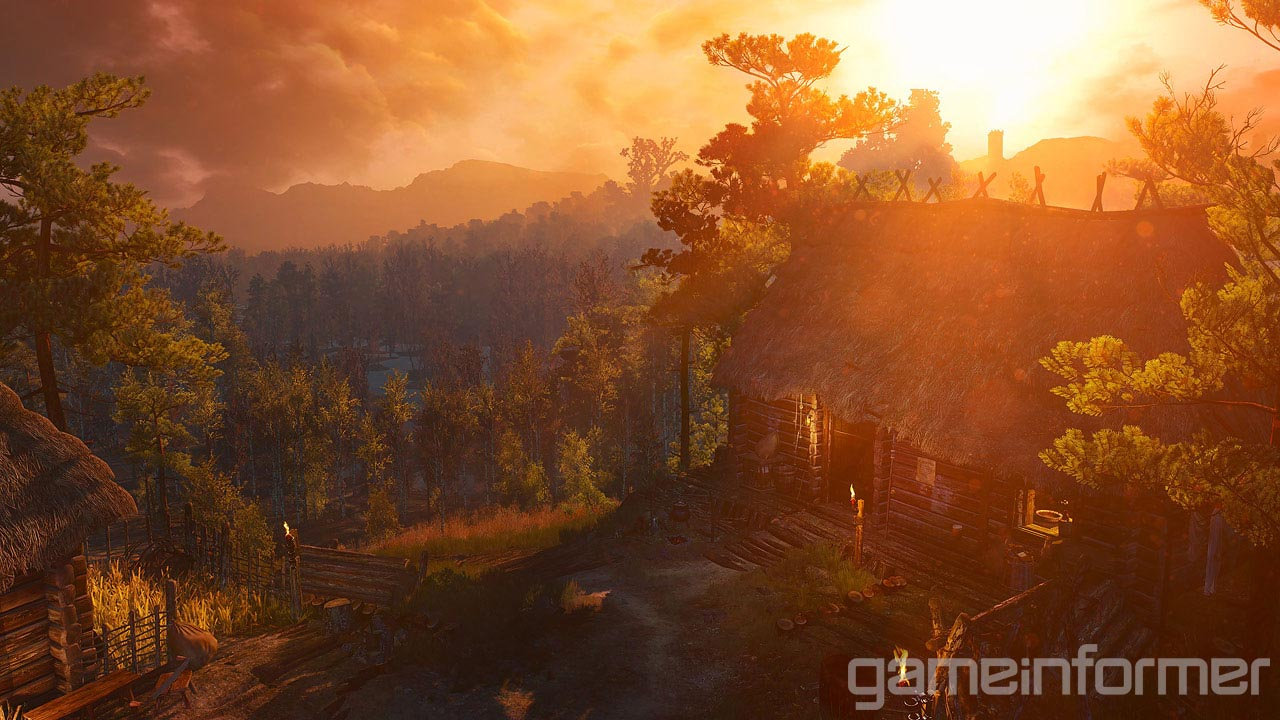
\includegraphics[scale=0.29]{images/einleitung/witcher_weather_1.jpg}
\caption{Grafik in \Fachbegriff{The Witcher 3: Wild Hunt}, Sonnenuntergang \cite{witcher_3_weather}}
\label{fig:witcher_weather_1}
\end{figure}

\begin{figure}[H]
\centering
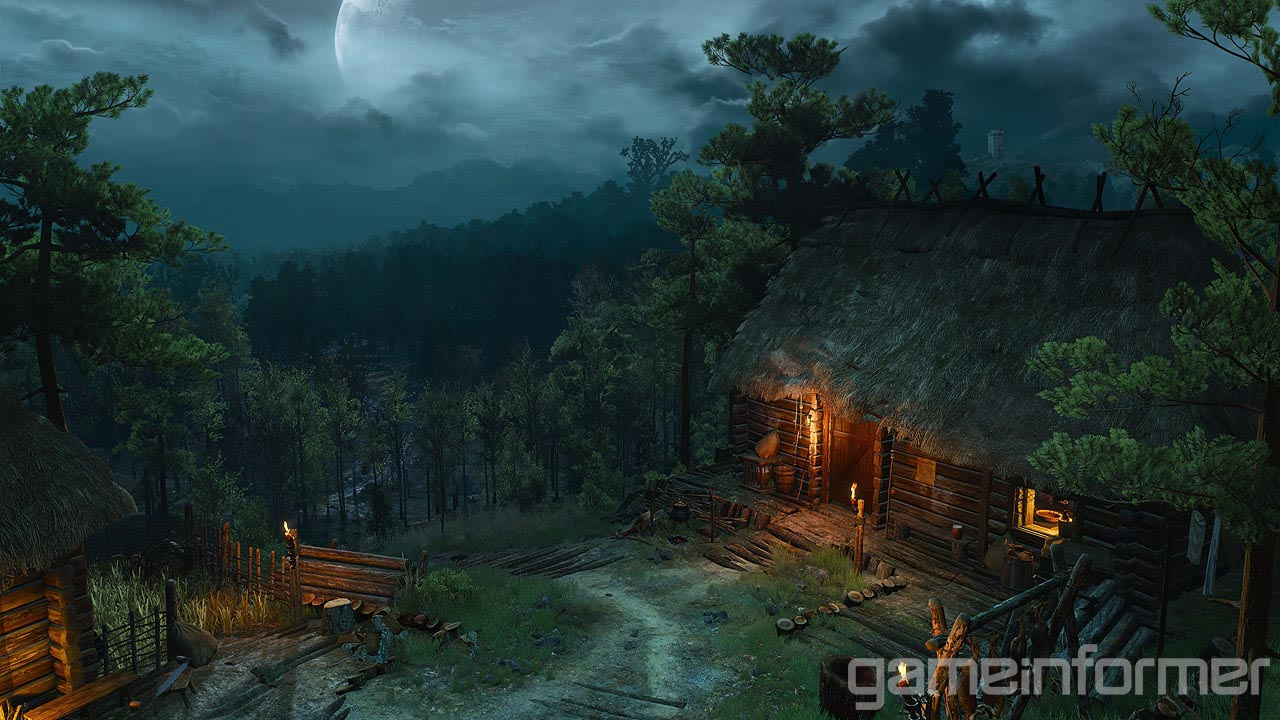
\includegraphics[scale=0.29]{images/einleitung/witcher_weather_2.jpg}
\caption{Grafik in \Fachbegriff{The Witcher 3: Wild Hunt}, Nacht \cite{witcher_3_weather}}
\label{fig:witcher_weather_2}
\end{figure}

Aufgrund der Größe der Städte im Vergleich zu Skyrim muss eine deutlich größere Menge von NPCs verwendet werden. Wegen der höheren Anzahl handelt es sich bei dem Großteil dieser NPCs um namenlose, unbekannte Charaktere. Eine festgelegte Anzahl bekannter NPCs würde hier nicht ausreichen, um die deutlich größere Spielwelt zu füllen. Begibt sich der Spieler an einen Ort, so werden diese Hintergrundcharaktere hinzugefügt und nach dem Verlassen des Ortes wieder entfernt. Diese dienen weniger dem Spielfortschritt sondern der Bevölkerung der Spielwelt. Besonders wegen der Anzahl der Charaktere fällt nicht sofort auf, dass diese stets die gleichen Aktivitäten ausüben. Verfolgt man hingegen einen NPC, so wird schnell ersichtlich, dass sehr einfache Handlungsmuster vorliegen, die sich stets wiederholen. Beispielsweise gehen \acp{npc} endlos zufällig durch die Stadt oder stehen kontinuierlich auf dem Markplatz, anstatt dass sie ihre Aktivitäten zu einem gewissen Zeitpunkt abbrechen, auf ihre Umwelt reagieren und eine neue, sinnvolle Tätigkeit suchen. Dadurch wird die Immersion der Spielwelt verringert. Die Agenten verfügen über keinen sinnvollen Tagesablauf, der mit ihren persönlichen Präferenzen oder Eigenschaften wie ihrem Alter, ihrem Geschlecht oder ihrem Beruf übereinstimmt. Um eine überzeugende Welt darzustellen verfügen Spieler über eine bestimmte Erwartungshaltung, die nicht vollständig erfüllt wird. Beispielsweise sollte ein NPC dem gefolgt wird nach einer gewissen Zeit seinen Wohnort erreichen, sich dann zur Abendzeit schlafen legen und anschließend morgens zur Arbeit gehen.

Die oben beschriebenen statischen Verhaltensmuster lassen sich trotz einer Zunahme der Immersion in anderen Bereichen in den meisten Spielen feststellen. Die vorliegende Arbeit fokussiert sich auf einen Lösungsansatz für diese zugrunde liegende Problematik. Dabei wird der Fokus nicht auf den visuellen Aspekt gelegt, sondern auf das Finden sinnvoller \ac{npc}-Aktionen und dem damit verbundenen Entscheidungsprozess. Ein möglichst menschlich wirkendes Verhalten soll durch eine sinnvolle Auswahl von Tätigkeiten vermittelt werden. Dabei wird ein Machine Learning-Ansatz gewählt, um statt aufwändigem Scripting einen Lernprozess der Agenten anzuregen, sodass weniger manuelle Arbeit nötig ist. Konkret sollen \acp{npc} entwickelt werden, die sich als Hintergrundcharaktere in einer entwickelten Dorfsimulation, um die Spieltwelt lebendig wirken zu lassen.

Das Verhalten der Agenten soll einen sinnvollen Tagesablauf abbilden, der von ihren Attributen, Bedürfnissen und z.B. dem Beruf des \ac{npc} abhängt. Sie erhalten eine Auswahl aus verschiedenen Aktionen, mit denen sie ihre Bedürfnisse befriedigen können, die auf grundsätzlichen menschlichen Bedürfnissen basieren. Dieses Vorgehen wird gewählt, weil gezeigt wurde, dass die Verwendung von menschlichen Eigenschaften wie Bedürfnissen zur Glaubwürdigkeit von Charakteren beitragen können \cite{fallon:believable_background_characters}. Konkret handelt es sich bei den verwendeten Bedürfnissen um interne Funktionen für Eigenschaften wie Hunger, Durst oder Kommunikation. Man spricht von \Fachbegriff{Utility Based Agents} (siehe Abschnitt \ref{utility_agents}). Weiterhin verfügen sie über statische Attribute wie Sportlichkeit, Kommunikationsfreudigkeit oder Intelligenz, die ihre Persönlichkeit definieren sollen. Generell soll dadurch ein möglichst menschliches Verhalten angeregt werden.

Im Folgenden wird kurz die jeweilige Thematik vorgestellt, mit der sich die einzelnen Kapitel der Thesis befassen.

\paragraph{Kapitel \ref{intelligente_agenten} - \nameref{intelligente_agenten}:}
Als erstes behandelt dieses Grundlagenkapitel die Funktionsweise intelligenter Agenten. Dabei werden unterschiedliche typische Verfahren beleuchtet, die für die Entwicklung intelligenter Agenten relevant sind.

\paragraph{Kapitel \ref{reinforcement_learning} - \nameref{reinforcement_learning}:}
\Fachbegriff{Reinforcement Learning} wird als ein Kernkonzept für die Entwicklung lernender Agenten vorgestellt. Zunächst wird dafür auf die generelle Verwendung maschinellen Lernens in Spielen eingegangen. Wichtige Grundlagen wie \Fachbegriff{Markov Decision Problems} werden näher erläutert. Die generelle Funktionsweise sowie der mathematische Hintergrund von modellfreien und modellbasierten Verfahren werden vorgestellt. Weiterhin werden ausgewählte relevante Algorithmen aus dem Bereich, insbesondere der in dieser Arbeit verwendete Algorithmus \ac{ppo}, erläutert. Zuletzt werden Beispiele zum State-of-the-Art von Reinforcement Learning beschrieben.

\paragraph{Kapitel \ref{ml_games_beispiele} - \nameref{ml_games_beispiele}:}
In diesem Kapitel werden verschiedene Anwendungsfälle für Machine Learning in Videospielen beschrieben und in Kategorien eingeteilt. Dabei wird der Fokus nicht nur auf intelligente Agenten, sondern auf generelle Lösungen für die Verbesserung der Authentizität von Spielwelten gelegt. Es soll gezeigt werden, dass es Anwendungsbereiche gibt, in der die Verwendung von Machine Learning Verbesserungen hinsichtlich des Immersionslevels von Spielwelten erzielen kann.

\paragraph{Kapitel \ref{ml_unity} - \nameref{ml_unity}:}
Das Kapitel geht auf die Entwicklung von lernenden intelligenten Agenten innerhalb der Game Engine \Fachbegriff{Unity} ein. Das Hauptthema ist hier die Einführung in das \Fachbegriff{ML-Agents Toolkit}-Framework inklusive der Erläuterung der wichtigsten Konzepte. Zur Veranschaulichung wird ein beispielhaftes Projekt entwickelt und vorgestellt, um wesentliche Aspekte sowie die wichtigsten Komponenten herauszustellen.

\paragraph{Kapitel \ref{entwicklung_dorf} - \nameref{entwicklung_dorf}:}
Der entwickelte Ansatz einer Dorfsimulation mit lernenden, bedürfnisbasierten Agenten wird in diesem Kapitel dokumentiert. Die Anforderungen und generellen Eigenschaften der Simulation werden zunächst beschrieben. Die Architektur des Verfahrens wird anschließend erst generell und dann im Detail vorgestellt. Das Resultat in Form des modellierten Dorfes mit der zugrunde liegenden Architektur sowie den entwickelten Agenten, die sich in der Dorfsimulation bewegen und Aktionen ausführen, werden vorgestellt.

\paragraph{Kapitel \ref{agenten_training} - \nameref{agenten_training}:}
In diesem Kapitel wird der Trainingsvorgang beschrieben, der für den Lernvorgang der Agenten nötig gewesen ist. Dabei wird der Ablauf besprochen, zugrunde liegende Theorien erläutert und Probleme sowie ihre Lösungen gezeigt. Weiterhin werden die Güteüberprüfung des Trainings diskutiert und die Ergebnisse des Trainings vorgestellt. Dabei spielt die Wahl der Hyperparameter sowie die Wahl der Belohnungen der Agenten eine kritische Rolle.

\paragraph{Kapitel \ref{weitere_ansaetze} - \nameref{weitere_ansaetze}:}
Zusätzlich zu dem auf \Fachbegriff{Reinforcement Learning} basierenden Ansatz wurden zwei weitere Verfahren für die Entwicklung intelligenter Agenten genutzt. Zunächst wird die Implementierung dieser Ansätze besprochen. Anschließend werden Unterschiede, Vorteile und Nachteile der drei entwickelten Verfahren untersucht.


\paragraph{Kapitel \ref{fazit} - \nameref{fazit}:}
Schlussendlich wird ein Fazit zur vorliegenden Arbeit getätigt. Es beginnt mit einer rückblickenden Zusammenfassung aller Kapitel. Es wird eine Bewertung der entwickelten Dorfsimulation und den lernenden Agenten vorgenommen. Generelle Probleme mit \Fachbegriff{Machine Learning} und \Fachbegriff{Reinforcement Learning} sowie spezifische Schwierigkeiten, die in der Thesis entstanden sind, werden diskutiert. Ein Ausblick soll schließlich Vorschläge zu Verbesserungsmöglichkeiten und weiterer Forschung geben. 

